\section{Chosen Solution}
To provide the project with valuable information about how the system could work in the real world, we also choose a solution for the hardware elements.
This is despite the fact that only the chosen software solution that is the website, the interfaces, and some simulated hardware elements is implemented.

For the availability of bicycles, we choose to use docks since it also covers part of the hardware aspect of a different requirement, being able to lock.  
For locking we also choose to use passwords that need to be input at the station because it is something everyone can do once the booking has been done, as SMS, QR codes, and GPS require phones and might not be suitable for tourists.
For tracking of bicycles we use GPS.

The following provides an overview of the chosen solution using rich pictures.

The server-station relationship is shown in \figref{fig:ServerRichPicture}.
It depicts a central server, where the different bicycle stations are connected to.
Furthermore, people can access the website to gain information e.g. bicycle count, but also to register bookings, where the server then communicates this to the given station(s).
Those stations then takes care of locking/unlocking bicycles to satisfy the bookings performed.
The server contains all information about each station, such as bookings, amount of available bicycles at stations, and usage statistics.
It provides booking and amount of available bicycles at stations through a website to the user. 
Usage statistics are provided to the facilitators of the system and gives them the ability to improve it. 

\begin{figure}[h]
\centering
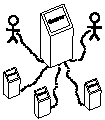
\includegraphics[scale=3]{serverrichpicture/server.pdf}
\caption{The server and the associated stations.}
\label{fig:ServerRichPicture}
\end{figure}

The dock that provide the locking/unlocking mechanism along with the bicycle detection ability have to talk to the station. 
This is for example when they need to unlock a booked bicycle, the information needs to be propagated from the station to the individual dock containing the bicycle.
A sketch of how a station could look like when deployed can be seen in \figref{fig:StationRichPicture}.
The figure depicts a station and two docks connected to the station, which contains a bicycle each. 
On the display of the station, it can be seen that two bicycles are available for use.
\begin{figure}[h]
\centering
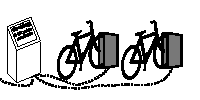
\includegraphics[scale=3]{stationrichpicture/station.pdf}
\caption{The station and the bikes.}
\label{fig:StationRichPicture}
\end{figure}